\documentclass[spanish,xcolor=table,svgnames]{beamer}
\definecolor{mediumpurple4}{rgb}{0.36,0.28,0.55}
%colores coporativos
\definecolor{naranja}{rgb}{0.86,0.42,0.06}
\definecolor{gris}{rgb}{0.41,0.41,0.41}
\definecolor{azul}{rgb}{0.06,0.31,0.55}
\definecolor{rojo}{rgb}{1,0,0}
\usecolortheme[named=azul]{structure}

\mode<presentation>
{

  \usetheme{Warsaw}
%\useoutertheme{infolines}
  \setbeamercovered{transparent}
  \setbeamertemplate{navigation symbols}{}
}
\usepackage{listings}
\usepackage{color}
\definecolor{gray97}{gray}{.97}
\definecolor{gray75}{gray}{.75}
\definecolor{gray45}{gray}{.45}
\usepackage{listings}
\lstset{ frame=Ltb,
     framerule=0pt,
     aboveskip=0.5cm,
     framextopmargin=3pt,
     framexbottommargin=3pt,
     framexleftmargin=0.4cm,
     framesep=0pt,
     rulesep=.4pt,
     backgroundcolor=\color{gray97},
     rulesepcolor=\color{black},
     %
     stringstyle=\ttfamily,
     showstringspaces = false,
     basicstyle=\small\ttfamily,
     commentstyle=\color{blue},
     keywordstyle=\bfseries,
     %
     numbers=left,
     numbersep=15pt,
     numberstyle=\tiny,
     numberfirstline = false,
     breaklines=true,
   }
 
% minimizar fragmentado de listados
\lstnewenvironment{listing}[1][]
   {\lstset{#1}\pagebreak[0]}{\pagebreak[0]}
 \lstdefinestyle{consola}
   {basicstyle=\scriptsize\bf\ttfamily,
    backgroundcolor=\color{gray75},
   }
\lstdefinestyle{consola}
   {basicstyle=\scriptsize\bf\ttfamily,
    backgroundcolor=\color{gray75},
   }

\lstdefinestyle{XML}
   {language=XML,
   }

\usepackage[spanish]{babel}
\usepackage[utf8x]{inputenc}
\usepackage{charter}
\usepackage[T1]{fontenc}
\usepackage{fancyvrb}
\usepackage{tikz}
%\usepackage{microtype}
\usepackage{xspace}
\usepackage{ctable}
\usepackage{alltt,multicol}

\newcommand{\reduce}{\fontsize{8}{9}\selectfont}
%\usetikzlibrary{chains,positioning,decorations.pathreplacing,fit,scopes}

\title[Apertura de datos en proyetos Django]{Apertura de datos en proyetos Django}
\author[José Manuel Llerena Carmona]{José Manuel Llerena Carmona\\Tutores: Iván Ruíz Rube y Juan Manuel Dodero Beardo}
\institute[UCA]{Ingeniería Informática  \\ Universidad de Cádiz}
\date{16 de diciembre de 2013}

\DefineVerbatimEnvironment{vrbwithcmd}{Verbatim}{commandchars=+(),fontsize=\small}

\begin{document}

\begin{frame}
  \titlepage
  \begin{figure}
	
\includegraphics[height=0.2\textheight]{logo_uca} 
  \end{figure}
\end{frame}

\frame{\frametitle{Índice}\tableofcontents}

%%%%%%%%%%%%%%%%%%%%%%%%%%%%%%%%%
\section{Introducción}
\begin{frame}{Introducción}
    \tableofcontents[currentsection]
\end{frame}

\subsection*{Motivación}
\begin{frame}{Motivación}
  \begin{columns}[onlytextwidth]
    \begin{column}{0.5\textwidth}
      \begin{block}{Motivación del proyecto}
        \begin{itemize}
          \item Actualidad: existen multitud de datos en la web.
          \item Necesidad de un formato común.
          \item Organizaciones interesadas en abrir sus datos.
          \item Existencia estándares y vocabularios.
          \item No existen aplicaciones para Django.
        \end{itemize}
      \end{block}
    \end{column}
    \begin{column}{0.5\textwidth}
      \centering
      \begin{figure}[H]
        \begin{center}
            
\includegraphics[width=0.6\textwidth]{img/rdf.png}
        \end{center}
        \label{fig:python}
      \end{figure}
    \end{column}
​  \end{columns}
\end{frame}


\subsection*{Alcance}
\begin{frame}{Alcance}
\begin{block}{Objetivo}
El objetivo principal del presente proyecto es el de proporcionar una
herramienta, la cual le permita al usuario realizar la apertura controlada de
los datos de su proyecto Django.
\end{block}
\end{frame}

\begin{frame}{Framework}
  \begin{block}{¿Qué es Django?}
  \begin{itemize}
    \item Es un framework de código abierto escrito en Python.
    \item Está orientado al desarrollo de aplicaciones web.
    \item Se basa en el patrón Modelo-Vista-Controlador.
    \item Mantenido por la Django Software Foundation (DSF).
    \item Orientado para la creación de sitios webs complejos.
  \end{itemize}
  \end{block}


  \begin{columns}[onlytextwidth]
    \begin{column}{0.5\textwidth}
      \centering
      \begin{figure}[H]
        \begin{center}
            
\includegraphics[width=0.7\textwidth]{img/django.png}
        \end{center}
        \label{fig:django}
      \end{figure}
    \end{column}
    \begin{column}{0.5\textwidth}
      \centering
      \begin{figure}[H]
        \begin{center}
            
\includegraphics[width=1.0\textwidth]{img/python.png}
        \end{center}
        \label{fig:python}
      \end{figure}
    \end{column}
​  \end{columns}
\end{frame}

\begin{frame}{Objetivos específicos}
\begin{block}{Objetivos específicos}
Para conseguir este objetivo principal, se deberán cumplir los siguientes sub-objetivos:
\begin{itemize}
    \item Resolución de modelos del proyecto.
    \item Interfáz de configuración de la apertura de datos.
    \item Herramientas para publicación de datos.
\end{itemize}
\end{block}
\end{frame}

%%%%%%%%%%%%%%%%%%%%%%%%%%%%%%%%%
\section{Planificación}
\frame{\frametitle{Planificación}\tableofcontents[currentsection]}

\subsection*{Metodología}
\begin{frame}{Metodología}
    \begin{center}
    \begin{figure}[H]
      \begin{center}
          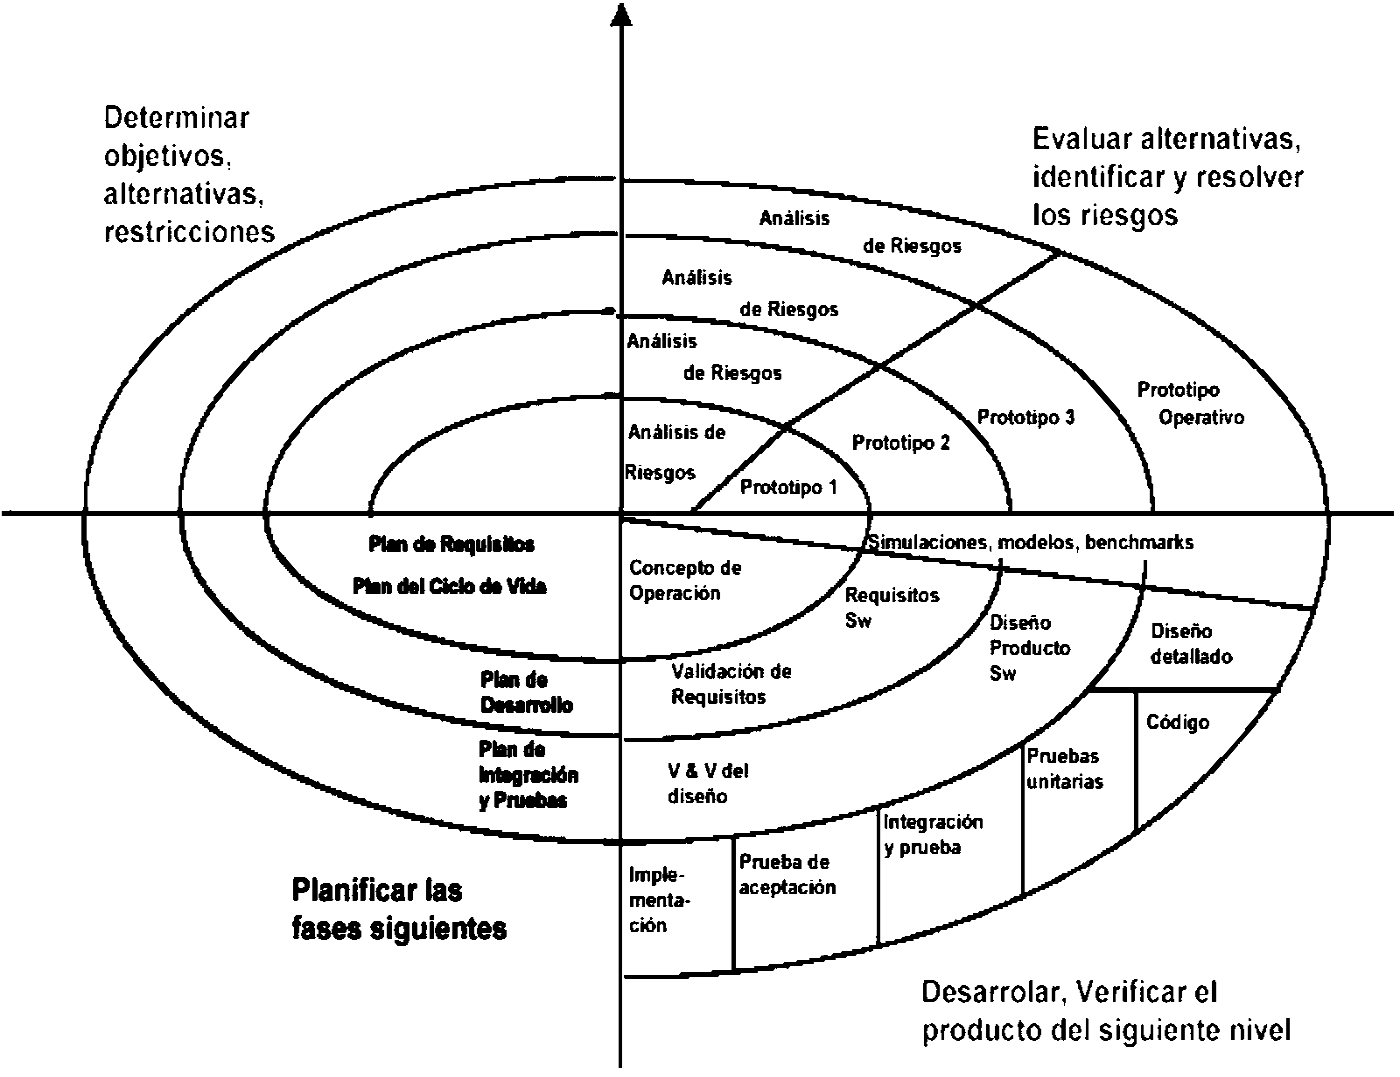
\includegraphics[width=0.8\textwidth]{img/espiral.png}
      \end{center}
      \label{fig:espiral}
    \end{figure}
  \end{center}
\end{frame}

\subsection*{Calendario}
\begin{frame}{Calendario}
  \begin{center}
    \begin{figure}[H]
      \begin{center}
          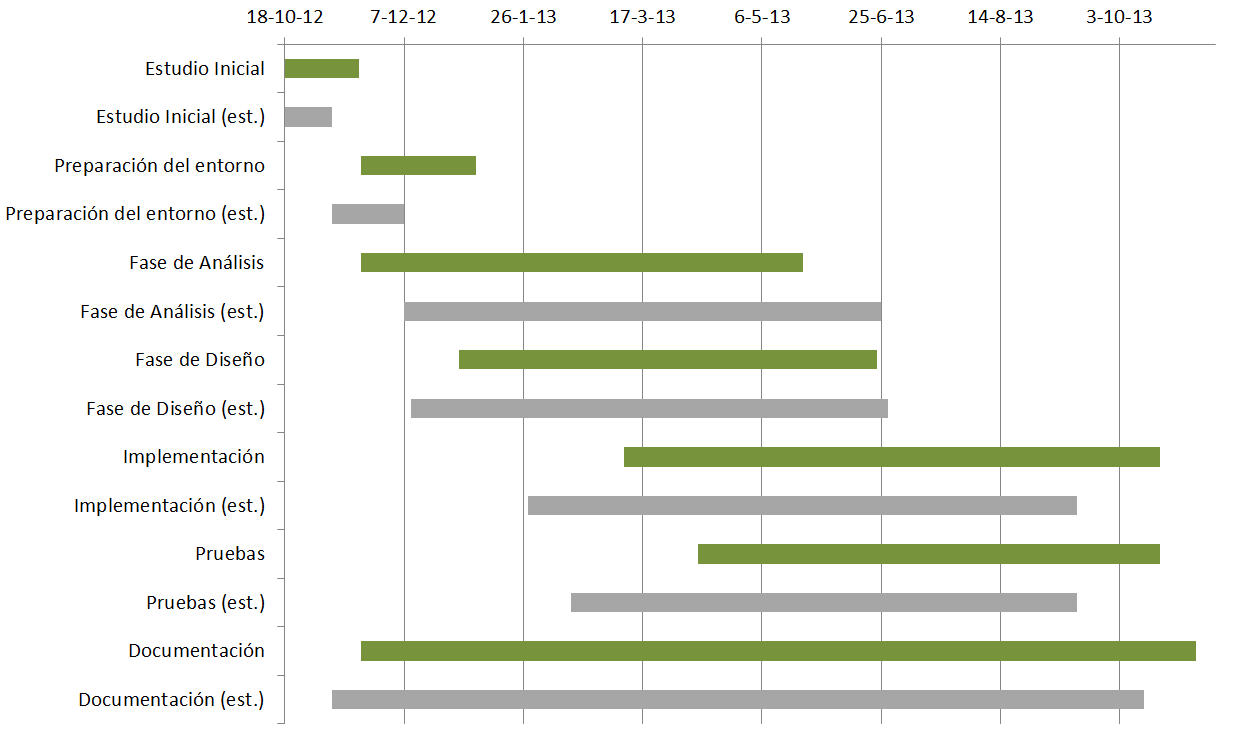
\includegraphics[width=1.0\textwidth]{img/diagrama_gantt.png}
      \end{center}
      \caption{Diagrama de Gantt con tiempos estimados}
      \label{fig:gantt}
    \end{figure}
  \end{center}
\end{frame}

% \subsection*{Costes}
% \begin{frame}{Costes}
%   \begin{center}
%     \begin{figure}[H]
%       \begin{center}
%           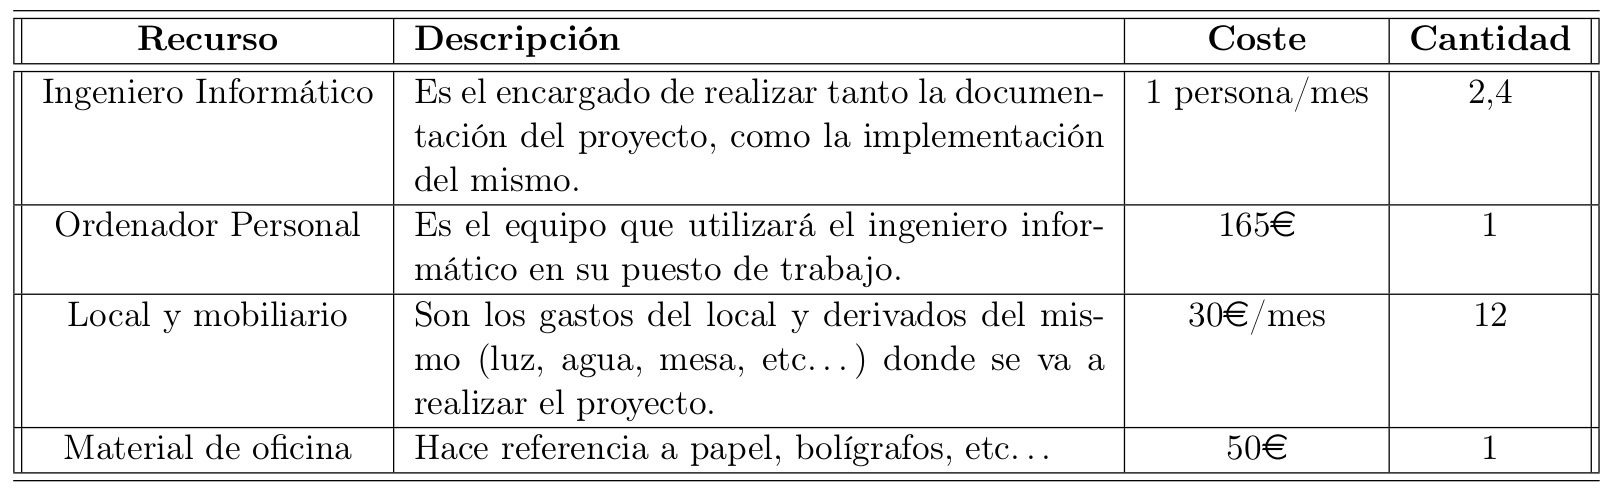
\includegraphics[width=1.0\textwidth]{img/coste1.png}
%       \end{center}
%       \label{fig:coste}
%     \end{figure}
%   \end{center}
% \end{frame}

%%%%%%%%%%%%%%%%%%%%%%%%%%%%%%%
\section{Desarrollo del proyecto}
\frame{\frametitle{Desarrollo del proyecto}\tableofcontents[currentsection]}

\subsection*{Análisis y requisitos}
\begin{frame}{Requisitos funcionales}
  \begin{figure}[H]
    \begin{center}
        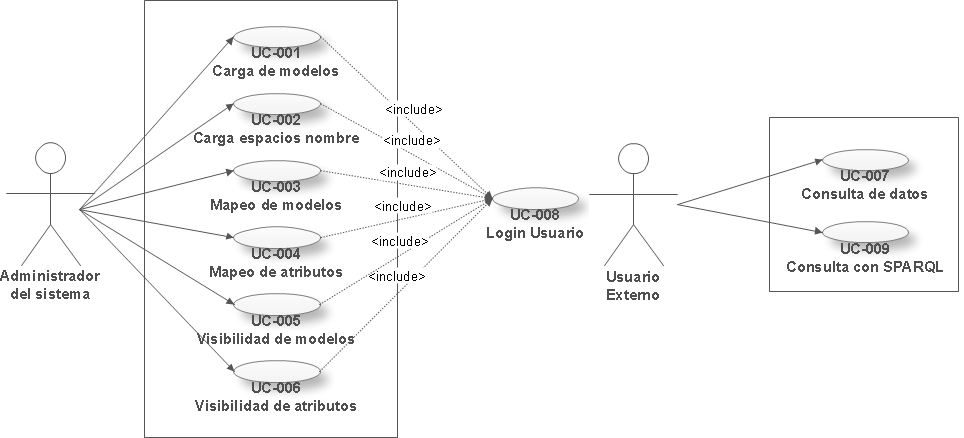
\includegraphics[width=1.0\textwidth]{img/casouso.png}
    \end{center}
    \label{fig:cu1}
  \end{figure}
\end{frame}


\begin{frame}{Requisitos de información}
  \centering
    \begin{figure}[H]
      \begin{center}
          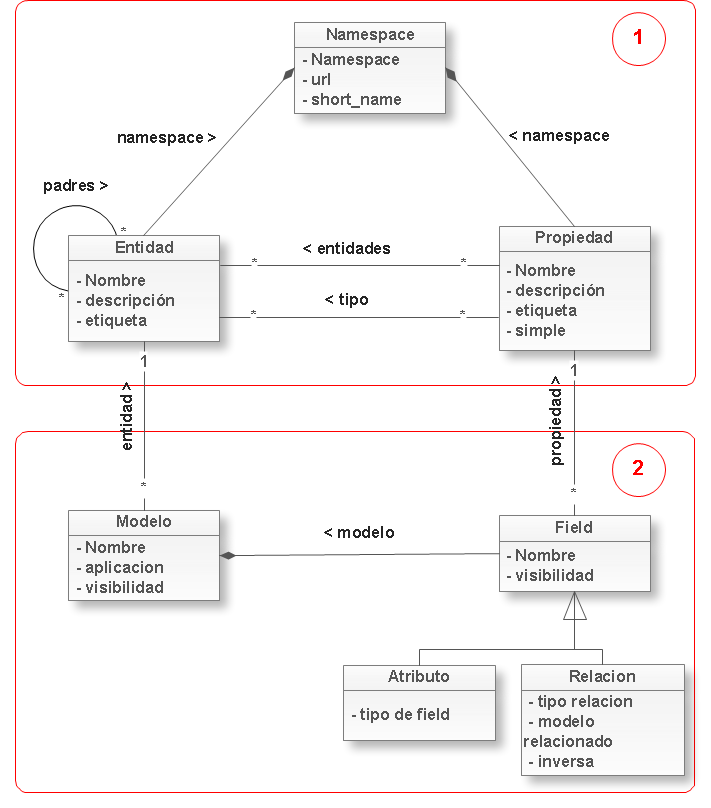
\includegraphics[width=0.54\textwidth]{img/diagrama_clases.png}
      \end{center}
      \label{fig:dia_clases}
    \end{figure}
\end{frame}

\begin{frame}{Requisitos no funcionales}
  \begin{block}{Requisitos no funcionales}
  \begin{itemize}
    \item Seguridad.
    \item Estándares de las organizaciones.
    \item Portabilidad.
    \item Mantenibilidad.
    \item Extensibilidad.
    \item Interfaz.
    \item Entorno tecnológico Django.
  \end{itemize}
  \end{block}
\end{frame}

\subsection*{Diseño}
\begin{frame}{Diseño interfaz de usuario}
  \begin{figure}[H]
    \begin{center}
      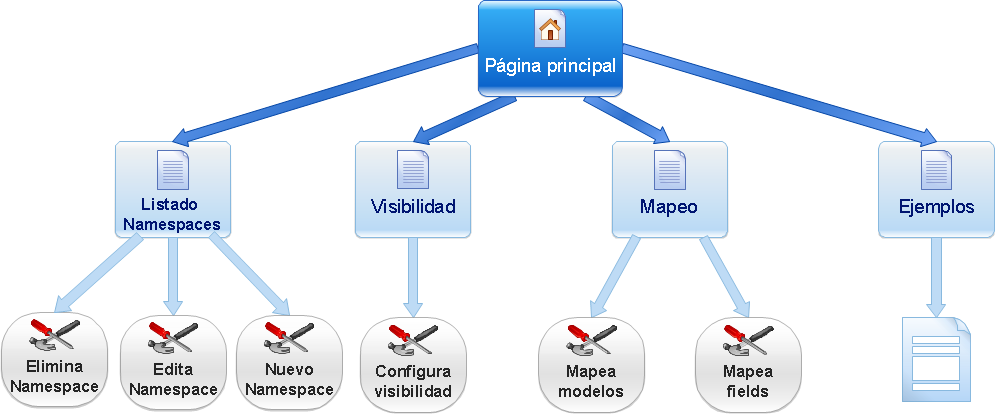
\includegraphics[width=1.0\textwidth]{img/mapa_web.png}
    \end{center}
    \label{fig:mapaweb}
\end{figure}
\end{frame}

\begin{frame}{Diseño interfaz de usuario}
  \begin{figure}[H]
  Se han realizado el prototipado de la aplicación web.
    \begin{center}
        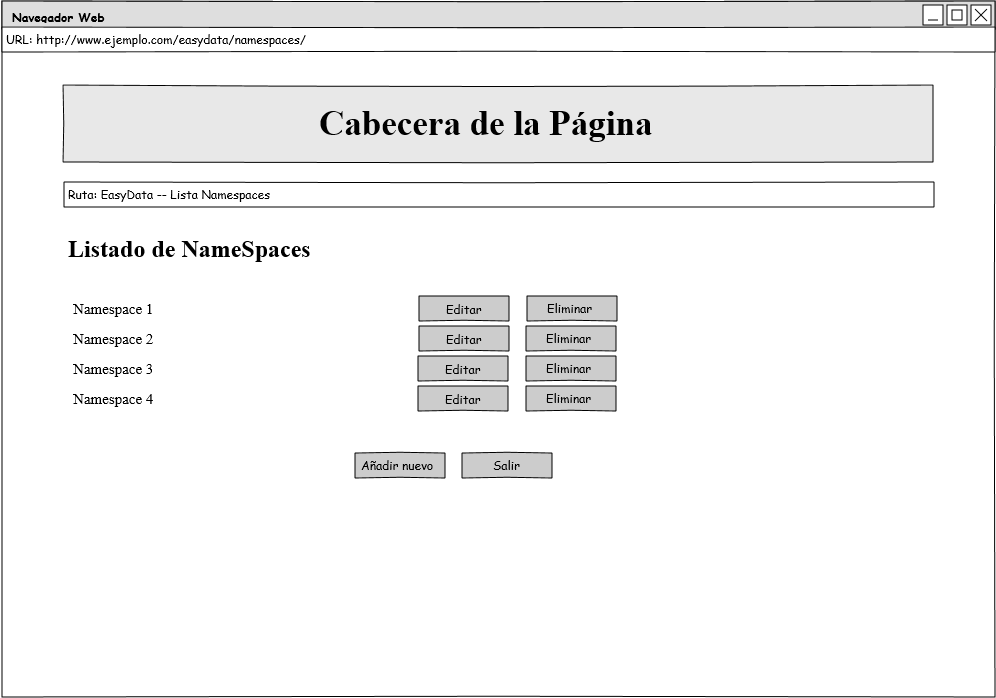
\includegraphics[width=0.7\textwidth]{img/lista_namespaces.png}
    \end{center}
    \label{fig:namespaces}
\end{figure}
\end{frame}

\begin{frame}{Diseño de los datos}
  \begin{figure}[H]
    \begin{center}
        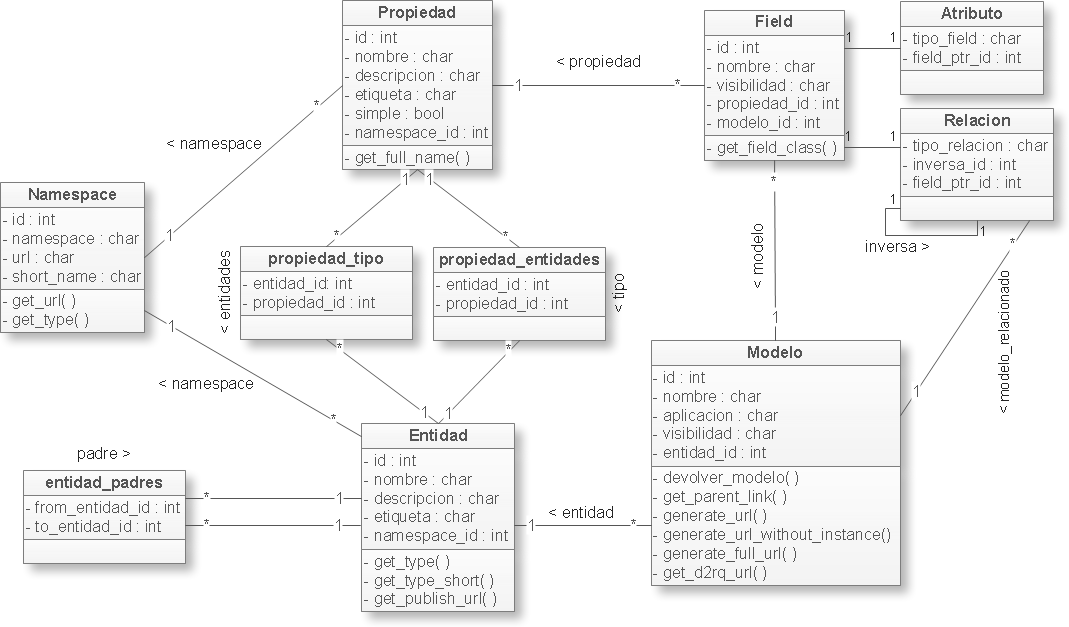
\includegraphics[width=1.0\textwidth]{img/modelo_conceptual.png}
    \end{center}
    \label{fig:conceptual}
\end{figure}
\end{frame}

\begin{frame}{Diseño de componentes}
  \begin{figure}[H]
    \begin{center}
        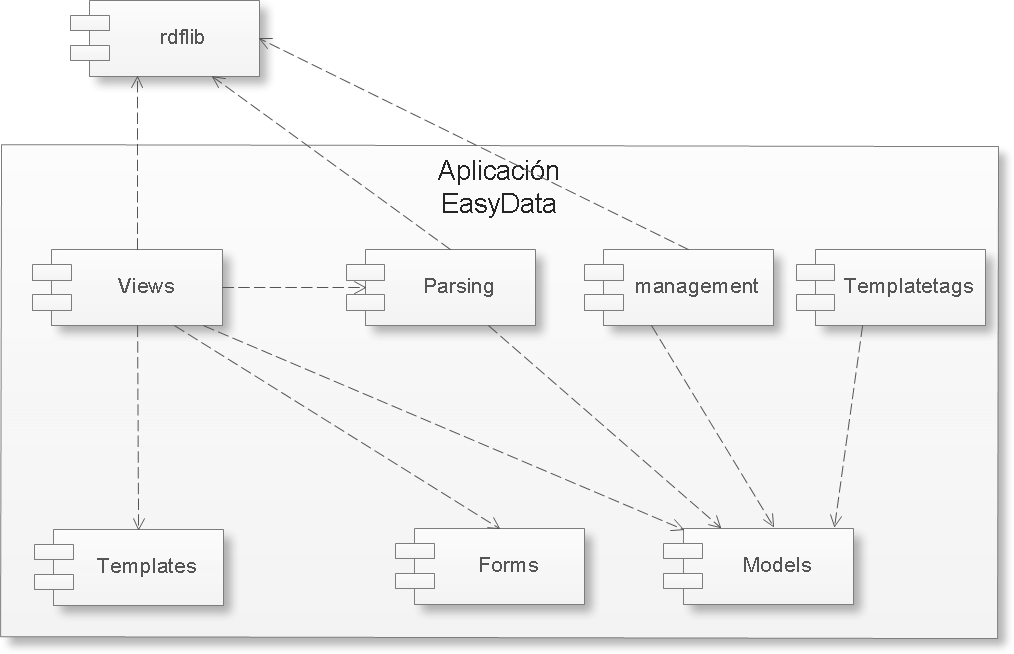
\includegraphics[width=0.8\textwidth]{img/estructura.png}
    \end{center}
    \label{fig:estructura}
\end{figure}
\end{frame}

\subsection*{Implementación}

\begin{frame}{Entorno tecnológico}
  \begin{figure}[H]
    \begin{center}
        
\includegraphics[width=0.75\textwidth]{img/logos_combinados.png}
    \end{center}
    \label{fig:tecnologias}
  \end{figure}
\end{frame}

\begin{frame}{Implementación}
  \begin{block}{Implementación de la aplicación}
    \begin{itemize}
      \item Internacionalización y localización.
      \item Guía de estilos PEP8.
      \item Herramienta para comprobación de código PyLint.
      \item Pruebas:
      \begin{itemize}
        \item automáticas del código
        \item manuales del sistema
        \item validación de formatos
      \end{itemize}
  \end{itemize}
  \end{block}
\end{frame}

%%%%%%%%%%%%%%%%%%%%%%%%%%%%%%%
\section{Demostración}
\begin{frame}{Demostración}
  \tableofcontents[currentsection]
\end{frame}

\begin{frame}{Demostración}
  \begin{center}
    \Huge{DEMOSTRACIÓN}
  \end{center}
\end{frame}


%%%%%%%%%%%%%%%%%%%%%%%%%%%%%%%
\section{Conclusiones}
\frame{\frametitle{Conclusiones}\tableofcontents[currentsection]}

\subsection*{Objetivos alcanzados}
\begin{frame}{Objetivos alcanzados}
\begin{block}{Los objetivos alcanzados han sido...}
  \begin{itemize}
    \item La aplicación es capáz de resolver y almacenar los modelos de los
      proyectos Django.
    \item Gestionar vocabularios y configuración de modelos.
    \item Herramientas para la publicación de datos.
    \item Se han cumplido los plazos.
  \end{itemize}
\end{block}
\end{frame}

\subsection*{Lecciones aprendidas}
\begin{frame}{Lecciones aprendidas}
\begin{block}{Valoración...}
  \begin{itemize}
    \item Se han adquirido mejores conocimientos tanto del lenguaje Python como
      del framework Django.
    \item Importancia de seguir una metodología de trabajo, realizar una
      planificación del proyecto y un análisis y diseño del mismo.
    \item Se han adquirido nuevos conceptos relacionados con la Web Semántica.
    \item Trabajado con nuevas tecnologías y herramientas como SPARQL, RDF o
      D2Rq.
    \item Se han adquirido buenas prácticas a la hora de programar en
      Python/Django.
  \end{itemize}
\end{block}
\end{frame}

\subsection*{Trabajo futuro}
\begin{frame}{Trabajo futuro}
\begin{block}{Trabajos futuros...}
El trabajo futuro en esta aplicación podría abarcarse desde diferentes frentes:
\begin{itemize}
\item Varias configuraciones simultáneas.
\item Consulta sobre la base de datos haciendo uso de SPARQL.
\item Ampliar formatos de exportación de datos.
\item Ampliar la disponibilidad a otros frameworks.
\end{itemize}
\end{block}
\end{frame}

\section{Bibliografía}
\begin{frame}{Bibliografía}
  \tableofcontents[currentsection]
\end{frame}

\begin{frame}{Bibliografía}
  \begin{thebibliography}{10}
    \beamertemplatebookbibitems
    \bibitem{12} DjangoFoundation. \emph{Web oficial del proyecto Django, https://www.djangoproject.com/}. 2013.
    \bibitem{20} Documentación oficial Python, http://www.python.org/, 2013.
    \bibitem{13} Bob DuCharme, Learning sparql, O’Reilly, 2011.
    \bibitem{14} Tom Heath and Christian Bizer, LinkedDataBook, http://linkeddatabook.com/editions/1.0/, 2011.
    \bibitem{21} Guido Van Rossum and Barry Warsaw, Style Guide for Python Code, http://www.python.org/dev/peps/pep-0008/, 2012.
    \bibitem{15} jQuery, Documentación oficial jQuery, http://api.jquery.com/, 2013.
    \bibitem{16} Twitter, Bootstrap V3, http://getbootstrap.com/, 2013.
    %\bibitem{bibliografia1}....
  \end{thebibliography} 
\end{frame}

\begin{frame}{Bibliografía}
  \begin{thebibliography}{10}
    \beamertemplatebookbibitems
    \bibitem{17} Documentación oficial D2Rq, http://d2rq.org/, 2013.
    \bibitem{18} Project FOAF, FOAF, http://www.foaf-project.org/, 2010.
    \bibitem{19} Google-Microsoft-Yahoo!, Schema, http://schema.org/, 2012.
    \bibitem{22} Martin Hepp, Good Relations, http://www.heppnetz.de/projects/goodrelations/, 2012.
    \bibitem{24} W3C OWL, OWL, http://www.w3.org/TR/owl-ref/, 2004.
    \bibitem{24} W3C Microdata, Microdata, http://www.w3.org/TR/microdata/, 2013.
    \bibitem{27} W3C RDF, RDF, http://www.w3.org/TR/rdf-primer/, 2004.
    %\bibitem{bibliografia1}....
  \end{thebibliography} 
\end{frame}

\begin{frame}{Bibliografía}
  \begin{thebibliography}{10}
    \beamertemplatebookbibitems
    \bibitem{28} W3C RDFa, RDFa, http://www.w3.org/TR/rdfa-syntax/, 2013.
    \bibitem{25} W3C RDFS, RDFS, http://www.w3.org/TR/rdf-schema/, 2004.
    \bibitem{26} Ministerio de Hacienda y Administraciones Públicas de España, MAGERIT V3, 2012.
    \bibitem{23} Infojobs, Salarios Infojobs, http://plandecarrera.infojobs.net/, 2013.
    %\bibitem{bibliografia1}....
  \end{thebibliography} 
\end{frame}


\appendix
\frame
{
  \begin{center}
    \Huge{Gracias por su atención}
  \end{center}
  \begin{center}
    \url{https://pypi.python.org/pypi/django-easydata/}
  \end{center}
}
\end{document}
